\chapter{DESARROLLO DE LA SOLUCIÓN}

Este capítulo describe el desarrollo técnico y metodológico aplicado para llevar a cabo el análisis de los datos en este proyecto. Cada sección detalla los pasos realizados, las herramientas empleadas y los enfoques metodológicos utilizados para lograr una representación visual y analítica de los datos de video obtenidos.

\section{Equipo utilizado}
A continuación se presenta una descripción detallada de las características del equipo de cómputo utilizado en el desarrollo del proyecto. Esto es relevante para replicar el análisis en condiciones similares.

\begin{table}[H]
    \centering
    \caption{Especificaciones del equipo utilizado}
    \begin{tabular}{p{5cm} p{8cm}} \hline
        \textbf{Característica} & \textbf{Especificación} \\ \hline
        Nombre del dispositivo & LAPTOP-OSCAR \\
        Procesador & AMD Ryzen 7 6800H con Radeon Graphics, 3.20 GHz \\
        RAM instalada & 16.0 GB (15.3 GB utilizable) \\
        Tipo de sistema & Sistema operativo de 64 bits, procesador basado en x64 \\
        Sistema operativo & Windows \\ \hline
    \end{tabular}
    \label{tabla:laptop}
\end{table}
\section{Especificaciones de Python}
Para este proyecto se utilizó la versión 3.12.4 de Python, cuyo entorno fue configurado para cumplir con los requisitos de las bibliotecas y módulos necesarios.

\begin{table}[H]
    \centering
    \caption{Especificaciones de Python utilizado}
    \begin{tabular}{p{5cm} p{8cm}} \hline
        \textbf{Característica} & \textbf{Especificación} \\ \hline
        Versión de Python & 3.12.4 \\
        Fecha de compilación & 6 de junio de 2024 \\ \hline
    \end{tabular}
    \label{tabla:python}
\end{table}

\section{Librerías}
Las librerías descritas a continuación fueron esenciales para las distintas etapas de procesamiento, análisis y visualización en este proyecto.

\begin{longtable}{p{4cm} p{11cm}}
    \caption{Descripción de Librerías Usadas en el Proyecto} \\ % Caption con numeración automática
    \hline
    \textbf{Librería} & \textbf{Descripción} \\
    \hline
    \endfirsthead
    
    \hline
    \textbf{Librería} & \textbf{Descripción} \\
    \hline
    \endhead
    
    \hline
    \endfoot
    
    \hline
    \endlastfoot
    
    \multicolumn{2}{c}{\textbf{Web Scraping y automatización}} \\
    \hline
    \texttt{time} & Proporciona funciones para gestionar el tiempo, como retrasos y mediciones de intervalos, útiles en sincronización de procesos y espera entre solicitudes. \\
    \texttt{os} & Facilita la interacción con el sistema operativo, como gestionar archivos y directorios, útil en automatización. \\
    \texttt{subprocess} & Ejecuta comandos del sistema desde Python, permitiendo interactuar con otros programas o scripts. \\
    \texttt{psutil} & Ofrece una interfaz para monitorear recursos del sistema (CPU, memoria) y gestionar procesos en segundo plano. \\
    \texttt{selenium} & Herramienta para automatización de navegadores, ideal para pruebas web y scraping de sitios dinámicos. \\
    \texttt{tqdm} & Crea barras de progreso en loops, útil para monitorear procesos largos. \\
    \hline
    
    \multicolumn{2}{c}{\textbf{Procesamiento de datos}} \\
    \hline
    \texttt{numpy} & Biblioteca fundamental para operaciones matemáticas y estructuras de datos de alto rendimiento, como arreglos multidimensionales. \\
    \texttt{pandas} & Ofrece estructuras de datos como DataFrames, ideales para manipulación y análisis de datos tabulares. \\
    \hline
    
    \multicolumn{2}{c}{\textbf{Procesamiento de imágenes}} \\
    \hline
    \texttt{cv2} & OpenCV, biblioteca de visión artificial para procesamiento y análisis de imágenes y video, común en proyectos de visión. \\
    \texttt{hog} & Función en \texttt{skimage.feature} para extracción de características en imágenes usando Histogramas de Gradientes Orientados (HOG). \\
    \hline
    
    \multicolumn{2}{c}{\textbf{Redes neuronales y Deep learning}} \\
    \hline
    \texttt{ResNet50} & Arquitectura de red preentrenada, común para extracción de características y clasificación en imágenes. Se importa desde \texttt{tensorflow.keras.applications}. \\
    \texttt{preprocessing} & Módulo en Keras para preprocesamiento de datos e imágenes, útil en preparación de datos para redes neuronales. \\
    \texttt{models} & API de Keras para crear y gestionar modelos, permitiendo el diseño de redes neuronales profundas. \\
    \hline
    
    \multicolumn{2}{c}{\textbf{Clustering y Machine learning}} \\
    \hline
    \texttt{KMeans} & Algoritmo de agrupamiento en \texttt{sklearn.cluster}, útil para clasificar datos en grupos similares. \\
    \texttt{metrics} & Módulo de \texttt{sklearn} que ofrece métricas para evaluar modelos y métodos de clustering. \\
    \texttt{PCA} & Método de reducción de dimensionalidad en \texttt{sklearn.decomposition}, que simplifica conjuntos de datos complejos. \\
    \hline
    
    \multicolumn{2}{c}{\textbf{Visualización}} \\
    \hline
    \texttt{matplotlib} & Biblioteca principal para visualización de datos, permite crear gráficos de varios tipos en Python. \\
    \hline
    
\end{longtable}



\section{Extracción de datos}

La extracción de datos fue un paso fundamental en este proyecto, ya que permitió obtener información relevante de videos publicados en YouTube para su posterior análisis. El proceso se llevó a cabo en diferentes etapas que abarcaron desde la recopilación de los enlaces de los videos, la descarga de los mismos, hasta la extracción de frames que fueron utilizados para generar descriptores de características mediante técnicas de visión computacional.

\subsection{Automatización de la búsqueda de videos en YouTube}

Para obtener los videos de interés, se realizó una búsqueda automatizada en YouTube utilizando la librería \texttt{Selenium}. El objetivo era filtrar noticias en vivo y limitar la cantidad de videos a descargar. La siguiente secuencia de pasos describe el proceso:

\begin{itemize}
    \item Se inició una sesión de navegador automatizada con Selenium, controlando el navegador Chrome.
    \item A través de interacciones programadas, se realizaron búsquedas con palabras clave específicas y se aplicaron filtros para obtener resultados de videos de un único día y de la duración suficiente.
    \item Los enlaces de los videos obtenidos fueron almacenados en una lista para ser descargados posteriormente.
\end{itemize}

\begin{figure}[H]
    \centering
    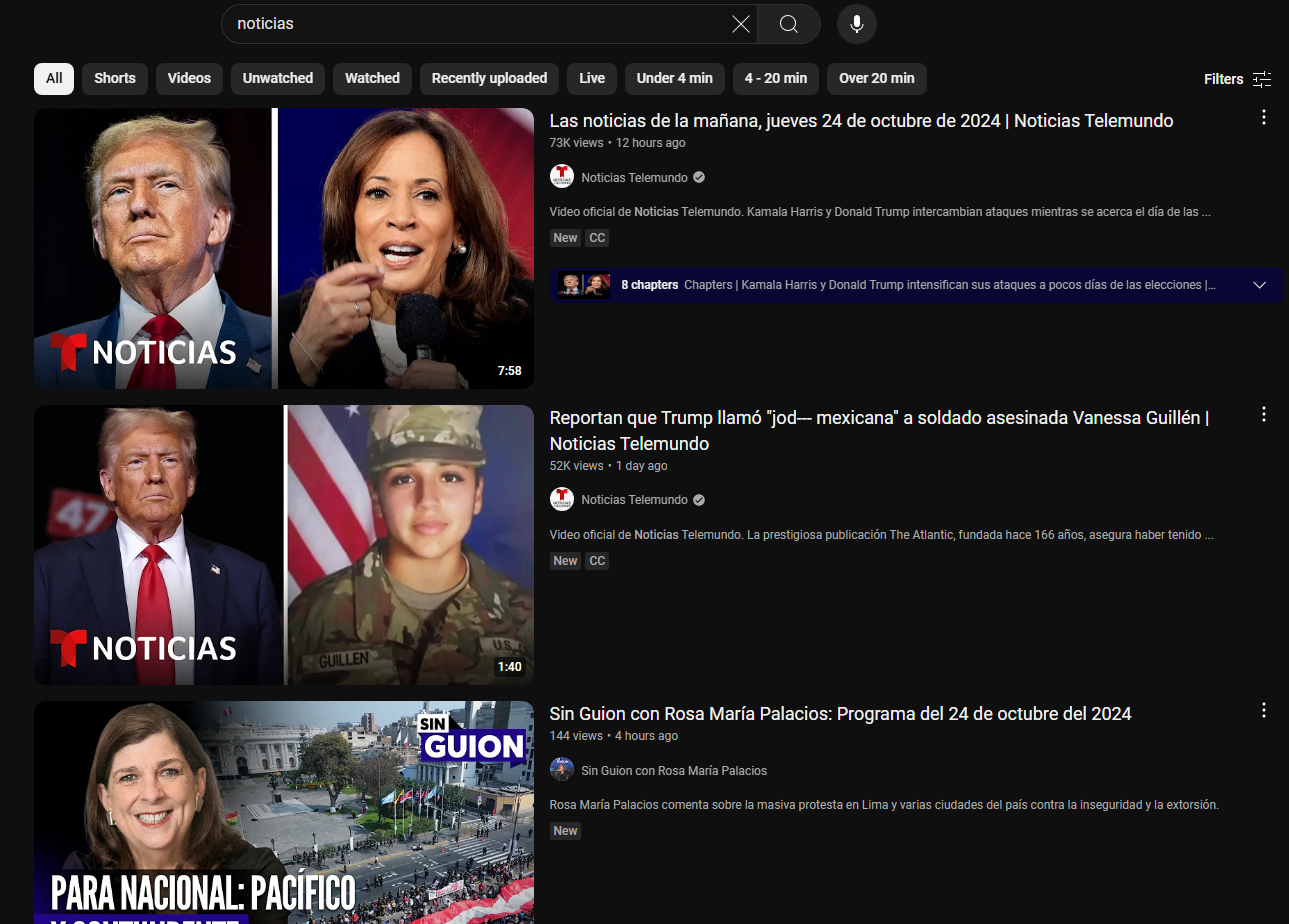
\includegraphics[width=0.70\textwidth]{4/figures/Extraccion_1.png}
    \caption{Página de partida de scrapping.}
    \label{fig:convolucion}
\end{figure}

\begin{figure}[H]
    \centering
    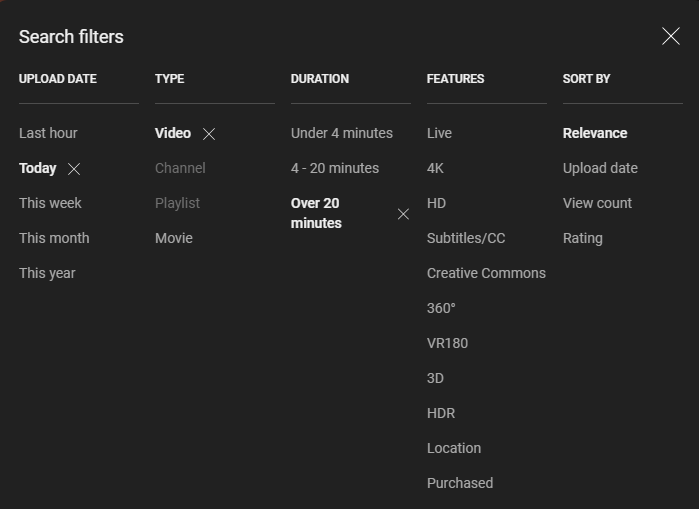
\includegraphics[width=0.70\textwidth]{4/figures/Extraccion_3.png}
    \caption{Filtros aplicados a los resultados de video.}
    \label{fig:convolucion}
\end{figure}

\subsection{Descarga de videos}

Para la recopilación de datos, se automatizó la descarga de videos de YouTube que cumplieran con los criterios. Para ello, se utilizó la herramienta \texttt{yt-dlp} estableciéndole los parámetros de descarga necesarios como el tamaño máximo de archivo y la calidad del video establecida en 720p.

El código de descarga inicializa una lista de enlaces de YouTube y ejecuta la descarga de cada video de forma secuencial, con un intervalo entre descargas para evitar bloqueos por parte de YouTube. A continuación, se detallan las opciones clave usadas con \texttt{yt-dlp}:

\begin{itemize}
    \item \texttt{--format "bestvideo[height<=720]"}: Especifica que se descargue la mejor calidad de video disponible con una altura máxima de 720 píxeles.
    \item \texttt{--max-filesize 400M}: Establece un tamaño máximo de archivo de 400 MB para evitar descargas excesivamente grandes.
\end{itemize}


\begin{figure}[H]
    \centering
    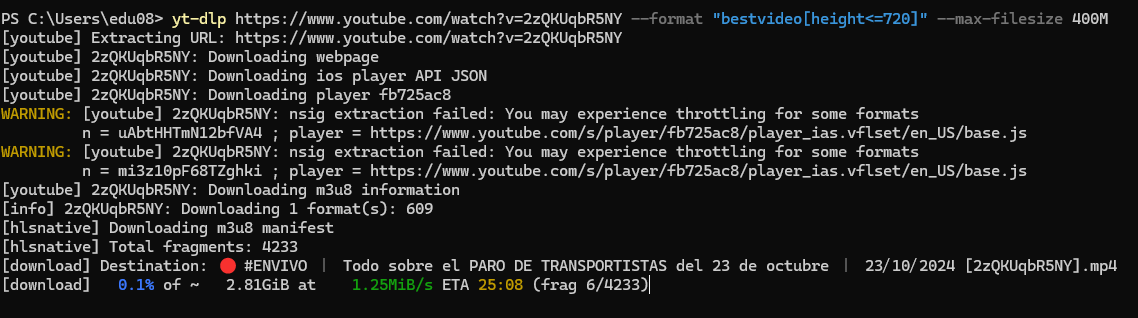
\includegraphics[width=0.90\textwidth]{4/figures/Descarga_1.png}
    \caption{Instrucción de descarga de video.}
    \label{fig:convolucion}
\end{figure}

\subsection{Organización de videos}

Para organizar los videos descargados, se empleó un script que clasifica los archivos en función de su tipo y ubicación en directorios específicos. Este proceso permite gestionar eficientemente los archivos de video y eliminar los archivos no necesarios generados durante la descarga. El procedimiento se detalla a continuación.

\begin{enumerate}
    \item \textbf{Creación del directorio de videos:} Inicialmente, se define un directorio específico para almacenar los archivos de video. Si la carpeta de destino no existe, el código se encarga de crearla utilizando el comando \texttt{os.makedirs}.
    
    \item \textbf{Clasificación de archivos:} Se definen las extensiones de archivo de video permitidas (\texttt{.mp4} y \texttt{.part}), las cuales son revisadas en cada archivo del directorio actual. Cualquier archivo con una de estas extensiones se mueve al directorio de videos.
    
    \item \textbf{Eliminación de archivos no necesarios:} Cualquier archivo que no corresponda a un video o al archivo \texttt{Tesis.ipynb} (notebook principal) es eliminado del directorio, optimizando el espacio y reduciendo el desorden en el sistema de archivos.
\end{enumerate}

Este proceso automatizado mejora la organización del proyecto y asegura que solo los archivos relevantes se mantengan en el directorio principal. En la investigación se obtuvieron 1.79 GB de contenido dividido en 15 videos de noticias.

\begin{figure}[H]
    \centering
    \includegraphics[width=0.40\textwidth]{4/figures/Organzación_1.png}
    \caption{Descripción final de carpeta de videos a procesar.}
    \label{fig:convolucion}
\end{figure}

\section{Preprocesamiento de datos}

El preprocesamiento de datos es un paso fundamental en este proyecto y consiste en cuatro etapas principales: la extracción de frames, el etiquetado de frames y las operaciones de transformación de los frames. Estas etapas permiten obtener representaciones visuales homogéneas y estructuradas, facilitando el análisis posterior mediante técnicas de machine learning.

\subsection{Extracción de frames}

La primera etapa del preprocesamiento es la extracción de frames de los videos. Los videos almacenados en la carpeta de entrada se procesan para obtener un conjunto de imágenes a intervalos de tiempo específicos, lo que permite captar información visual a lo largo de la duración del video. La extracción de frames se realiza a una tasa de \texttt{1 frame por segundo}, lo cual proporciona una representación balanceada entre resolución temporal y carga de procesamiento. Este proceso se logra utilizando la biblioteca \texttt{OpenCV}.

\subsection{Etiquetado de frames}

Cada frame extraído se etiqueta de manera única para mantener una referencia clara de su video de origen y posición temporal. La nomenclatura de los frames es de la forma \texttt{Video\{número\}\_Frame\{número\}.png}, donde:
\begin{itemize}
    \item \texttt{Video\{número\}} hace referencia al identificador del video de origen.
    \item \texttt{Frame\{número\}} indica el número de frame dentro del video.
\end{itemize}

Esta estructura de nombres facilita el seguimiento de cada frame y permite una asociación directa entre la imagen y el video de origen. En etapas posteriores se hará uso de la etiqueta para la identificación de frames clave y la generación de clips.

\begin{figure}[H]
    \centering
    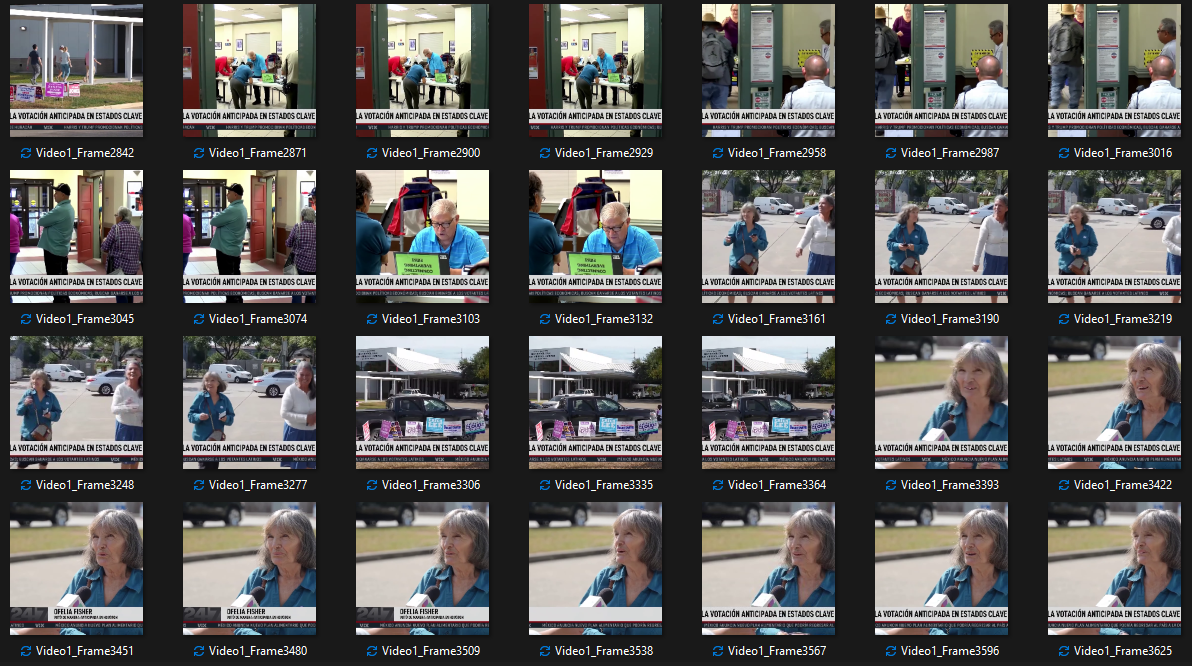
\includegraphics[width=0.80\textwidth]{4/figures/Etiquetado_1.png}
    \caption{Frames etiquetados en la carpeta de frames.}
    \label{fig:convolucion}
\end{figure}

\subsection{Operaciones sobre los frames}

Para garantizar la uniformidad en los datos y preparar los frames para su posterior análisis, cada imagen extraída de los videos pasa por un proceso de redimensión y recorte. Estos ajustes son esenciales para normalizar el tamaño de los frames y preservar la proporción original de la imagen, evitando así posibles distorsiones que puedan afectar los resultados en etapas posteriores del procesamiento.

El tamaño final de cada frame se define en \texttt{224x224 píxeles}, un formato ampliamente compatible con redes neuronales convolucionales (CNNs) y modelos de aprendizaje profundo en general. Este proceso de preprocesamiento se realiza en dos pasos clave:

\begin{itemize}
    \item \textbf{Redimensión}: Inicialmente, la imagen es escalada para que su dimensión menor (ancho o alto) se ajuste al tamaño objetivo de \texttt{224 píxeles}. Esto asegura que la imagen completa se mantenga dentro del marco sin deformaciones y preservando la proporción de los elementos visuales originales.
    \item \textbf{Recorte}: Una vez redimensionada, la imagen es recortada para ajustar la dimensión restante a \texttt{224 píxeles}, logrando así un encuadre preciso sin distorsionar los contenidos importantes. 
\end{itemize}


\begin{figure}[H]
    \centering
    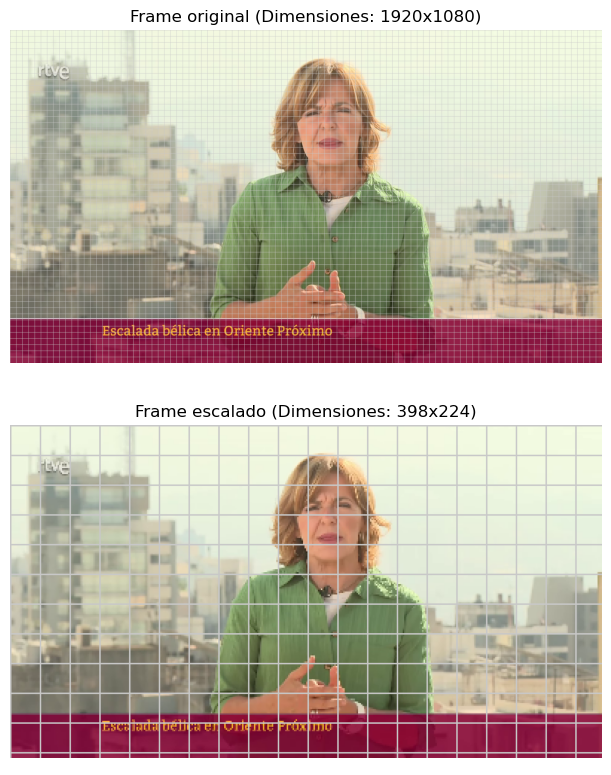
\includegraphics[width=0.50\textwidth]{4/figures/Preprocesamiento_1.png}
    \caption{Proceso de redimensión de la imagen.}
    \label{fig:preproc-resize}
\end{figure}

La Figura~\ref{fig:preproc-resize} ilustra la etapa de redimensión, mientras que la Figura~\ref{fig:preproc-crop} muestra el proceso de recorte, donde se enmarca la sección central de la imagen para asegurar consistencia en el análisis de los frames.

\begin{figure}[H]
    \centering
    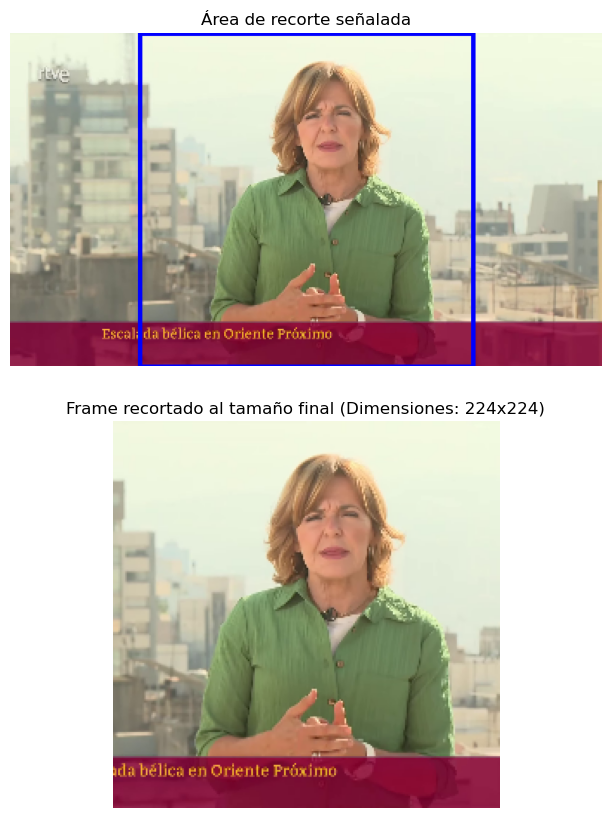
\includegraphics[width=0.30\textwidth]{4/figures/Preprocesamiento_2.png}
    \caption{Proceso de recorte de la imagen.}
    \label{fig:preproc-crop}
\end{figure}



\subsection{Guardado de frames}

Finalmente, los frames procesados se almacenan en un directorio de salida específico, asegurando que cada imagen esté etiquetada de forma clara y sea fácilmente localizable para su análisis posterior. Los frames resultantes se guardan en formato \texttt{.png}, manteniendo una alta calidad de imagen sin compresión excesiva que podría comprometer la precisión en las etapas de análisis.

\begin{figure}[H]
    \centering
    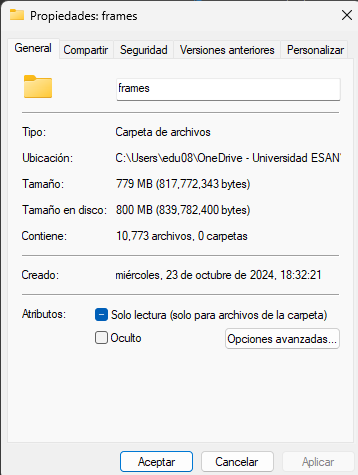
\includegraphics[width=0.40\textwidth]{4/figures/Guardado_1.png}
    \caption{Características principales de la carpeta de frames generada.}
    \label{fig:convolucion}
\end{figure}

Este proceso generó más de 10000 frames uniformes y etiquetados listos para el proceso de Extracción de características.

\section{Extracción de características}
La extracción de características es esencial para la representación compacta de la información visual en imágenes, permitiendo la realización de tareas analíticas avanzadas. En esta sección se describen los métodos de extracción y combinación de características utilizados: Histogram of Oriented Gradients (HOG) y Convolutional Neural Networks (CNN) con el modelo ResNet50 preentrenado en ImageNet, y el proceso de concatenación para unir las características de ambas técnicas.

\subsection{HOG (Histogram of Oriented Gradients)}

El método HOG se implementa en este proyecto como una técnica avanzada de extracción de características visuales, transformando cada frame en histogramas de gradientes de orientación. Este enfoque permite identificar contornos y texturas esenciales en los datos de imagen, evitando la necesidad de redundar en descripciones del proceso detallado, el cual ya ha sido expuesto en la sección teórica sobre \textit{extracción de características} (ver sección \ref{sec:preprocesamiento_imagenes}). En esta fase de análisis, HOG contribuye de manera significativa al modelado de patrones visuales, resultando especialmente efectivo en la representación de información estructural crítica para el análisis de patrones y el agrupamiento de datos visuales.

La Figura~\ref{fig:preproc-crop} ilustra el proceso de conversión de cada imagen en un descriptor HOG, enfatizando la metodología aplicada para generar estos histogramas de gradientes orientados que sintetizan las características visuales fundamentales de cada frame. 

\begin{figure}[H]
    \centering
    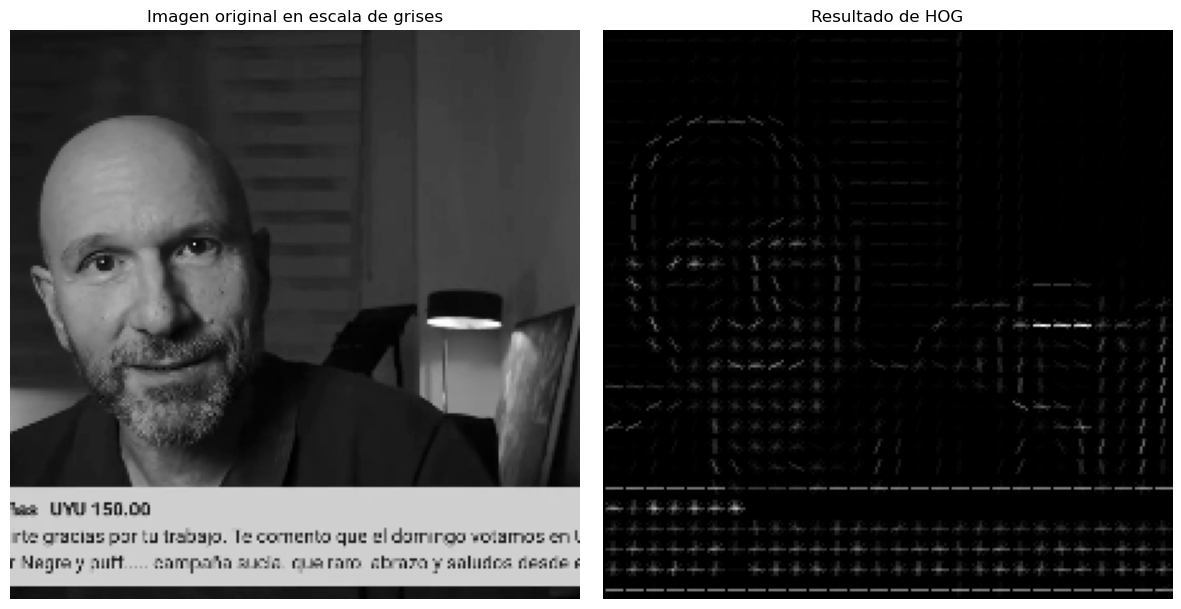
\includegraphics[width=0.60\textwidth]{4/figures/HOG_1.png}
    \caption{Proceso de transformación de imagen utilizando HOG.}
    \label{fig:preproc-crop}
\end{figure}

Los descriptores HOG obtenidos se integran en un \texttt{DataFrame}, el cual vincula cada frame con su correspondiente vector de características. Esta estructura, mostrada en la Figura~\ref{fig:convolucion}, no solo facilita la organización y accesibilidad de los datos, sino que también optimiza el procesamiento subsecuente. Al estructurar los datos en un formato tabular, el \texttt{DataFrame} permite un análisis más eficiente y la implementación de técnicas de machine learning en etapas posteriores del proyecto, asegurando una base de datos visualmente rica y ordenada para las siguientes fases del análisis.

\begin{figure}[H]
    \centering
    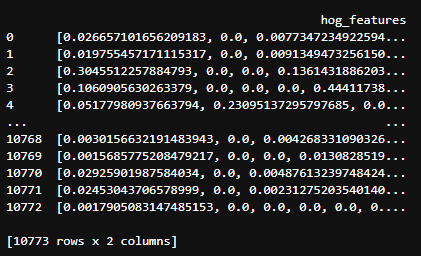
\includegraphics[width=0.60\textwidth]{4/figures/Caracteristicas_1.png}
    \caption{Estructura del DataFrame con los vectores de características HOG generados.}
    \label{fig:convolucion}
\end{figure}


\subsection{Extracción de características con CNN}
Para complementar la extracción HOG, se utiliza un modelo convolucional preentrenado (ResNet50) para extraer características de nivel más alto que capturan información estructural y semántica. la función extrae el vector de características de la capa \texttt{avg\_pool}, produciendo un descriptor de características CNN.

\begin{figure}[H]
    \centering
    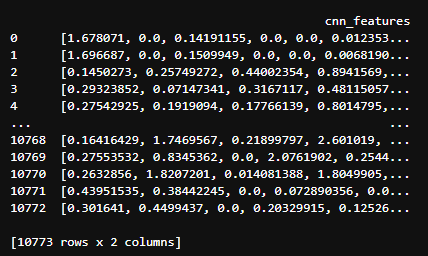
\includegraphics[width=0.60\textwidth]{4/figures/Caracteristicas_2.png}
    \caption{Dataframe generado por la red convolucional entrenada.}
    \label{fig:convolucion}
\end{figure}

\subsection{Concatenación de características}
Para maximizar la información obtenida a través de HOG y CNN, los vectores de características de ambas técnicas se integran en un único vector mediante un proceso de concatenación. Esta integración se realiza alineando ambos conjuntos de características de acuerdo con el identificador del frame y concatenando los vectores en una nueva columna denominada \texttt{combined\_features} dentro del \texttt{DataFrame} final, generando así una representación robusta de cada frame.

\begin{figure}[H]
    \centering
    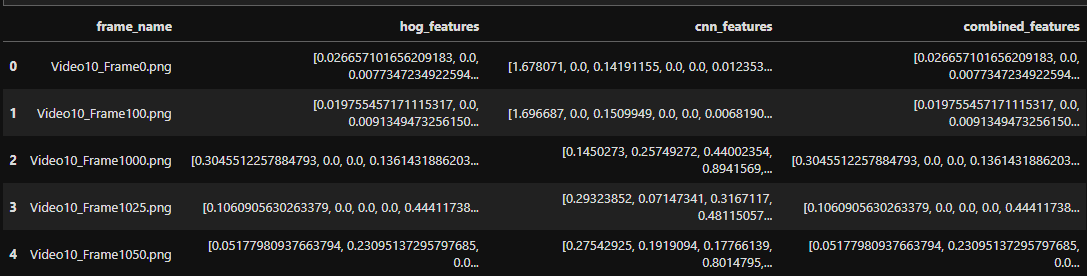
\includegraphics[width=0.70\textwidth]{4/figures/Caracteristicas_3.png}
    \caption{Concatenación de los vectores de características.}
    \label{fig:convolucion}
\end{figure}

Este \texttt{DataFrame} resultante, \texttt{merged\_df}, incluye las siguientes columnas:
\begin{itemize}
    \item \textbf{frame\_name}: El nombre del frame correspondiente.
    \item \textbf{hog\_features}: El vector de características HOG extraído.
    \item \textbf{cnn\_features}: El vector de características CNN extraído.
    \item \textbf{combined\_features}: Un vector de características unificado que contiene tanto HOG como CNN, lo que proporciona una representación robusta y rica de cada frame.
\end{itemize}

\section{Clasificación de datos}
Para organizar y analizar los datos obtenidos mediante extracción de características, se aplica un proceso de reducción de dimensionalidad seguido de un algoritmo de clustering. A continuación, se detallan los pasos para la clasificación y organización de datos.

\subsection{Reducción de dimensionalidad con PCA}
Dado que los vectores de características combinados (HOG + CNN) pueden ser de alta dimensión, aplicamos Principal Component Analysis (PCA) para reducirlos a 50 componentes principales, manteniendo la mayoría de la variabilidad de los datos. Esta reducción permite un análisis más manejable y mejora el rendimiento de algoritmos de clustering como K-means.

El método del codo se empleó para determinar el número óptimo de clusters, variando el valor de \( k \) y observando la inercia para distintos valores. La inercia representa la suma de distancias cuadradas desde cada punto hasta su centroide. 


\begin{figure}[H]
    \centering
    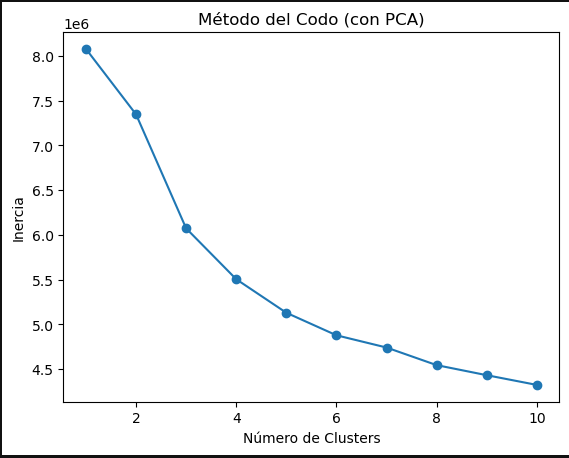
\includegraphics[width=0.60\textwidth]{4/figures/Modelo_4.png}
    \caption{Representación de la Inercia utilizando el método del codo.}
    \label{fig:convolucion}
\end{figure}


\subsection{Aplicación de K-means}

Una vez definido el número óptimo de clústeres, se aplica el algoritmo de K-means al conjunto de datos que contiene las características combinadas de Histogram of Oriented Gradients (HOG) y Convolutional Neural Networks (CNN). Este proceso permite agrupar los frames en categorías o clústeres específicos, basados en patrones de similitud en sus características visuales.

Para cada frame en el conjunto de datos, K-means asigna una etiqueta de clúster que indica a cuál grupo pertenece. Esta asignación se integra en el \texttt{DataFrame} original, permitiendo así un análisis estructurado de cada frame dentro de su grupo correspondiente.

\begin{figure}[H]
    \centering
    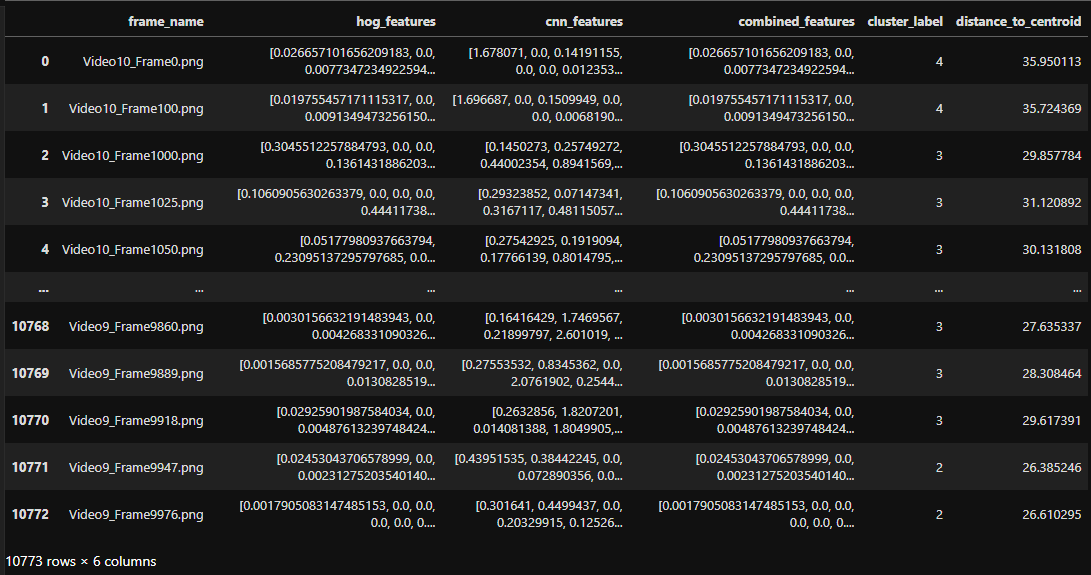
\includegraphics[width=0.80\textwidth]{4/figures/KNN_1.png}
    \caption{Asignación de clusters y distancias al centroide correspondiente.}
    \label{fig:convolucion}
\end{figure}

Además de la etiqueta de clúster, el algoritmo calcula la distancia de cada frame al centroide de su clúster. Esta distancia es fundamental para determinar el grado de representatividad de cada frame dentro de su grupo. Los frames más cercanos al centroide se consideran más representativos del clúster, mientras que aquellos a mayor distancia pueden representar características menos comunes. Esta información se incluye como una columna adicional en el \texttt{DataFrame} y es utilizada en análisis posteriores, como la selección de frames clave para la generación de clips representativos.


\subsection{Selección de frames clave}
Para cada cluster, identificamos los frames más representativos, es decir, aquellos más cercanos a los centroides, y los almacenamos en la lista \texttt{frames\_clave}.

Los frames seleccionados como representativos de cada cluster se muestran en una única imagen combinada. Esto proporciona una vista consolidada de los elementos clave de cada cluster.

\begin{figure}[H]
    \centering
    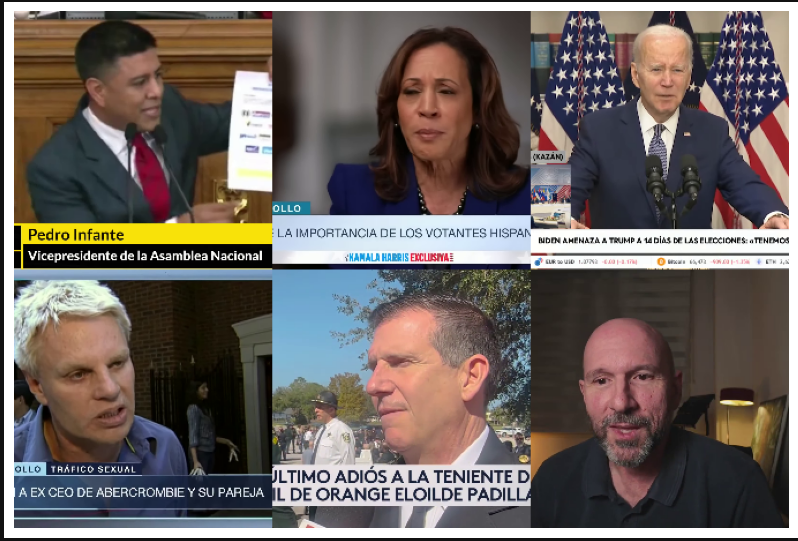
\includegraphics[width=0.60\textwidth]{4/figures/Frames_1.png}
    \caption{Características principales de la carpeta de frames generada.}
    \label{fig:convolucion}
\end{figure}

\section{Generación de Clips a partir de Frames Clave}

En esta sección se detalla el proceso de generación de clips de video basados en frames clave seleccionados en el análisis de clusters. Este proceso permite crear un video final que resalta los eventos representativos, proporcionando un contexto visual adicional para cada frame clave.

\subsection{Descripción del Proceso}
El proceso de generación de clips se lleva a cabo en tres etapas principales:

\begin{itemize}
    \item \textbf{Identificación de frame clave}: Cada frame clave se asocia con un video específico y se establece un rango de frames adyacentes a ese frame clave, seleccionado en base a la distancia temporal del evento destacado.
    \item \textbf{Selección de frames adyacentes}: Se seleccionan un conjunto de frames anteriores y posteriores al frame clave. Esto permite capturar el contexto visual necesario para proporcionar una vista completa del evento.
    \item \textbf{Combinación de clips}: Los clips individuales, correspondientes a cada frame clave y sus frames adyacentes, se concatenan en un solo video continuo que representa una síntesis de los eventos clave.
\end{itemize}

\subsection{Visualización de Resultados}
La Figura \ref{fig:clip_muestra} muestra el clip generado a partir de frames clave y sus frames adyacentes, destacando la coherencia visual que resulta de esta selección.

\begin{figure}[H]
    \centering
    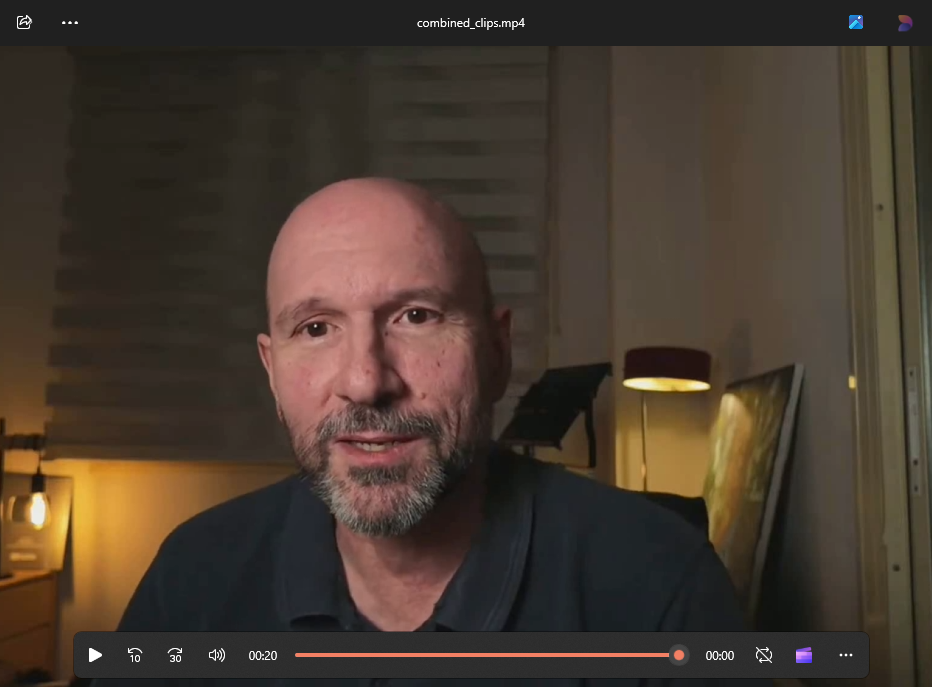
\includegraphics[width=0.8\textwidth]{4/figures/Clip_1.png}
    \caption{Muestra de frames clave y sus frames adyacentes.}
    \label{fig:clip_muestra}
\end{figure}

La Tabla \ref{tab:video_info} presenta un resumen de las especificaciones del video generado.

\begin{table}[H]
    \centering
    \caption{Especificaciones del Video Generado a partir de Frames Clave}
    \begin{tabular}{l c}
        \hline
        \textbf{Atributo} & \textbf{Valor} \\
        \hline
        Nombre del Video & combined\_clips.mp4 \\
        Resolución & 1920x1080 \\
        Duración (s) & 20.22 \\
        FPS & 29.97 \\
        \hline
    \end{tabular}
    \label{tab:video_info}
\end{table}

